\documentclass{article}

\usepackage{graphicx}
\usepackage{subcaption}
\usepackage{tikz}
\usepackage[utf8]{inputenc}
\usepackage[T1]{fontenc}
\usepackage{lmodern}
\usepackage{amsmath}
\usepackage{amsthm}
\usepackage{amsfonts}
\usepackage{amssymb}
\usepackage{enumitem}
\usepackage{commath}
\usepackage{mathtools}
\usepackage{adjustbox}
\usepackage{setspace}
\usepackage{bigints}
\usepackage{hyperref}
\usepackage{ulem}
\usepackage{esdiff}
\usepackage{pgfplots}
\usepackage{caption}
\usepackage{tikz-cd}
\usetikzlibrary{shapes.symbols}

\newtheorem{definicija}{Definicija}
\newtheorem{trditev}{Trditev}
\newtheorem{lema}{Lema}
\newtheorem{posledica}{Posledica}
\newtheorem{opomba}{Opomba}
\newtheorem{primer}{Primer}
\newtheorem{izrek}{Izrek}


\newcommand{\C}{\mathbb{C}}
\newcommand{\D}{\mathbb{D}}
\newcommand{\Z}{\mathbb{Z}}
\newcommand{\N}{\mathbb{N}}
\newcommand{\M}{\mathcal{M}}
\newcommand{\F}{\mathcal{F}}
\newcommand{\R}{\mathbb{R}}
\newcommand{\Ho}{\mathcal{O}}
\newcommand{\dd}{\mathrm{d}}


\title{Dinamika kompleksnih funkcij}
\author{Uroš Kosmač}

\begin{document}
\maketitle

V tem poglavju bomo obravnavali dinamiko holomorfnih funkcij
$f: D\subseteq \C \rightarrow \C.$ Ponovimo nekaj osnovnih pojmov.
\begin{definicija}
Množica $D \subseteq \C$ je \textbf{območje}, če je odprta in povezana.
\end{definicija}

\begin{opomba}
Območja so lahko neomejena ali omejena, ter enostavno povezana 
(brez lukenj) ali $m$-povezana ($m$ lukenj).
\end{opomba}

\begin{definicija}
Množica 
$$
\D(a, r) = \{z\in \C \,|\, |z - a| < r\}
$$
je disk in $\D = \D(0, 1)$ enotski disk.
\end{definicija}

\begin{definicija}
Funkcija $f: D\subseteq \C \rightarrow \C$ je holomorfna v $z\in D$ oz. na 
$D$, če obstaja limita 
\begin{equation}
f'(z) = \lim_{h\rightarrow 0} \frac{f(z + h) - f(z)}{h}.
\end{equation}
Množico holomorfnih funkcij na $D$ označimo z $\Ho(D)$.
\end{definicija}

Če kompleskno funkcijo zapišemo kot 
$$
f(z) = u(z) + iv(z) = u(x, y) + iv(x, y) \,\, \text{ za } \,\, u, v\in C^1(D)
$$
je $f\in \Ho(D)$ natanko tedaj, ko velja Cauchy-Riemannov sistem 
enačb:
\begin{equation}
u_x = v_y \,\,\text{ in }\,\, u_y = -v_x.
\end{equation}
Praksi so to običajno tiste, ki ne vsebujejo $\bar{z}$.
\noindent
Družina holomorfnih funkcij je precej "toga" oz. 
zanje veljajo razmeroma stroge omejitve in lastnosti 
\begin{itemize}
    \item Cauchyjeva integracijska formula: za $f\in \Ho(D) \cap C(\overline{D})$
    imamo 
    \begin{equation}
    f(z) = \frac{1}{2\pi i} \int_{\partial D} \frac{f(w)}{w - z} \dif w.
    \end{equation}
    To pomeni, da so vrednosti funkcije v notranjosti, določene z vrednostmi na robu.
    \item Holomorfne funkcije so $\C$-analitične t.j. 
    $$
    \forall a\in D. \exists r > 0: f(z) = \sum_{n=0}^\infty c_n(z- a)^n \,\, \text{ na }\,\, \D(a, r).
    $$
    Posledično so neskočnokrat odvedljive in so odvodi znova holomorfni.
    \item Njihova množica ničel je diskretna, tj. za ničlo 
    obstaja okolica, da na njej ni druge ničle. Če je $D$ omejena, 
    je ničel končno mnogo.
    \item Princip indentičnosti: če sta $f\in \Ho(D_f)$ in $g\in \Ho(D_g)$
    ter je $f = g$ na množici s stekališčem. Potem je 
    $f \equiv g $ na $D_f \cap D_g$. 
    \item Holomorfne funkcije so odprte. 
\end{itemize}

\begin{primer}
Osrednja primera 
\hfill 
\begin{enumerate}
    \item[i)] Polinomi: 
    $$
    p(z) = C_d z^d + C_{d-1} z^{d-1} + \dots + C_0, \,\, c_j \in \C, \,\, d = \text{deg}(p). 
    $$
    Imajo natanko $d$ ničel štetih z večkratnostjo. 
    \item[ii)] Racionalne funkcije: 
    $$
    f = \frac{p(z)}{q(z)} = \frac{C_d z^d + C_{d-1} z^{d-1} + \dots + C_0}{B_d z^d + B_{d-1} z^{d-1} + \dots + B_0},
    $$
    kjer sta $p, q$ polinoma. Imajo deg$(p)$ ničel in deg$(q)$ polov., stopnjo 
    pa definiramo kot deg$(f) = \max\{\text{def}(p), \text{def}(q)\}$.
\end{enumerate}
\end{primer}
\noindent
Kompleksno ravnino lahko kompaktificiramo z eno točko, kar nam da \textbf{Riemannovo sfero} $\hat{\C} = \C \cup \{\infty\}$.\\

\makeatletter 
\tikzset{ 
reuse path/.code={\pgfsyssoftpath@setcurrentpath{#1}} 
} 
\tikzset{even odd clip/.code={\pgfseteorule}, 
protect/.code={ 
\clip[overlay,even odd clip,reuse path=#1] 
(current bounding box.south west) rectangle (current bounding box.north east)
; 
}} 
\makeatother 
\usetikzlibrary{3d,arrows.meta,decorations.markings,perspective}
\tikzset{->-/.style={decoration={% https://tex.stackexchange.com/a/39282/194703
  markings,
  mark=at position #1 with {\arrow{>}}},postaction={decorate}},
  ->-/.default=0.55}

\pgfmathsetmacro{\myaz}{11}
\begin{tikzpicture}[declare function={%
        stereox(\x,\y)=2*\x/(1+\x*\x+\y*\y);%
        stereoy(\x,\y)=2*\y/(1+\x*\x+\y*\y);%
        stereoz(\x,\y)=(-1+\x*\x+\y*\y)/(1+\x*\x+\y*\y);
        Px=1.75;Py=-1.5;Qx=-1.5;Qy=-1.25;amax=2.5;},scale=2.5,
        line join=round,line cap=round,
        dot/.style={circle,fill,inner sep=1pt},>={Stealth[length=1.2ex]}]
 \pgfdeclarelayer{background} 
 \pgfdeclarelayer{foreground} 
 \pgfsetlayers{background,main,foreground}
 \path[save path=\pathSphere,ball color=gray,fill opacity=0.6] 
    (0,0) circle[radius=1];
 \begin{scope}[3d view={\myaz}{12}]
  \draw (-amax,amax) -- (-amax,-amax) coordinate (bl) -- (amax,-amax) 
  coordinate (br)-- (amax,amax)
  %node[above left]{$z=0$}
  ;
  \begin{scope}
   \tikzset{protect=\pathSphere}
   \draw (-amax,amax) -- (amax,amax);
  \end{scope}
  \begin{scope}
   \clip[reuse path=\pathSphere];
   \draw[dashed] (-amax,amax) -- (amax,amax);
  \end{scope}
  \begin{scope}[canvas is xy plane at z=0]
   \draw[dashed] (\myaz:1) arc[start angle=\myaz,end angle=\myaz+180,radius=1];
   \draw (\myaz:1) arc[start angle=\myaz,end angle=\myaz-180,radius=1];
   \path[save path=\pathPlane] (\myaz:amax) -- (\myaz+180:amax) --(bl) -- (br) -- cycle;
   \begin{scope}
   %\begin{pgfonlayer}{background}   
    \clip[use path=\pathPlane];
    \draw[dashed,use path=\pathSphere];
   %\end{pgfonlayer}
   \end{scope}
   \begin{scope}
    \tikzset{protect=\pathPlane}
    \draw[use path=\pathSphere];
   \end{scope}
   \begin{pgfonlayer}{background}
    \fill[blue!30,fill opacity=0.6]
     (\myaz:1) arc[start angle=\myaz,end angle=\myaz-180,radius=1]
     -- (-amax,0) -- (-amax,amax) -- (amax,amax) -- (amax,0) -- cycle;
   \end{pgfonlayer}
   \fill[blue!30,fill opacity=0.6]
     (\myaz:1) arc[start angle=\myaz,end angle=\myaz-180,radius=1]
     -- (-amax,0) -- (-amax,-amax) -- (amax,-amax) -- (amax,0) -- cycle;
  \end{scope}
  \draw[->-=0.3] (Px,Py,0) node[dot,label=below:{$w$}](w){}
  -- node[auto,pos=0.3,swap]{$\pi$} ({stereox(Px,Py)},{stereoy(Px,-1)},{stereoz(Px,Py)})
   node[dot,label=below left:{$w^*$}](w*){};
  \draw[->-] (Qx,Qy,0) node[dot,label=below:{$z$}](z){}
  -- node[auto,pos=0.5]{$\pi$} ({stereox(Qx,Qy)},{stereoy(Qx,-1)},{stereoz(Qx,Qy)})
   node[dot,label=below right:{$z^*$}](z*){};
  \begin{pgfonlayer}{background} 
   \draw[dashed] (w*) -- (0,0,1) node[dot,label=above:{$\zeta$}](zeta){}
   -- (z*) -- (w*);
  \end{pgfonlayer} 
  \draw (2,1.5) node[anchor=south] {$\C$};
 \end{scope}
\end{tikzpicture}
Obnašanje $f$ v okolici $z = \infty$ analiziramo tako, da 
uporabimo konjugacijo s preslikavo $z\mapsto \frac{1}{z}$
na $\C\slash \{0 \}$. Ta nam vrednost $z = \infty$ prevede 
na izhodišče. Pravimo, da je $f$ holomorfna na okolici $z = \infty$, 
če je taka $f\left(\frac{1}{z}\right)$ na okolici $z = 0$.
\begin{primer}
\begin{enumerate}
\hfill
\item[i)] $f(z) = \frac{1}{z - 1}$  
\begin{align*}
&f(1) = \infty \Longrightarrow \,\,\text{ pogledamo } \,\, \frac{1}{f(z)} = z - 1 \Longrightarrow \,\,z=1 \text{ je pol $1$. stopnje}\\
&f(\infty) = 0 \Longrightarrow \,\, \text{ pogledamo }\,\, f\left( \frac{1}{z}\right) = \frac{1}{\frac{1}{z} - 1} = \frac{z}{1 - z} = z + z^2 + \dots \Longrightarrow \text{ $z = \infty$ je ničla $1$.stopnje}
\end{align*}
\item[ii)] $f(z) = z^2 + 1$
$$
f(\infty) = \infty \Longrightarrow \,\, \text{ pogledamo }\,\, \frac{1}{f\left( \frac{1}{z}\right)} = \frac{1}{\frac{1}{z^2} + 1} = \frac{z^2}{1 + z^2} = z^2 + z^4 + \dots \Longrightarrow \text{ $z = \infty$ je pol $2$.stopnje}
$$
\item[iii)] $f(z) = e^z = e^x(\cos{y} + i\sin{y})$. Vrednosti 
$f(\infty)$ nemoremo smiselno definirati, sa velja 
\begin{align*}
\lim_{x\rightarrow -\infty} e^{x + iy} &= 0 \\
\lim_{x\rightarrow \infty} |e^{x + iy}| &= \lim_{x\rightarrow \infty} e^{x} = \infty.
\end{align*}
\end{enumerate}
\end{primer}

\begin{izrek}
Funkcija $f: \hat{\C} \rightarrow \hat{\C}$ je holomorfna natanko tedaj, ko je razširitev racionalne funkcije ali $f \equiv \infty$.
\end{izrek}

\begin{proof}[Dokaz:]
~\\
$(\Longleftarrow)$: sledi iz primerov.\\ 
$(\Longrightarrow)$: 
Za funkcijo, ki jo lahko holomorfno razširimo na $\hat{\C}$, velja:
\begin{enumerate}
\item[i)] če $f\in \Ho(\C)$ nima polov in $f(\infty) \neq \infty$ je po Liouvillovem izreku konstantna, saj je omejena.
\item[ii)] če ima $f$ na $\C$ neskončno mnogo polov, potem zaradi diskretnosti, obstaja zaporedje le teh, ki gre proti $\infty$.
Posledično bo tudi $f(\infty) = \infty$ in zaradi zveznosti in $f \equiv \infty$ zaradi principa identičnosti.
\item[iii)] Če ima $f$ le končno mnogo polov, ima po podobnem argumentu, kot pri $ii)$ tudi končno mnogo ničel. Potem definiramo $R$, racionalno funkcijo z istimi ničlami in poli. 
Po $i)$ je $\frac{f}{R}$ konstantna.
\end{enumerate}
Povzetek: takoj ko ima $f$ neskočno ničel ali polov oz. kako bistveno singularnost, je nemoremo obravnavati na $\hat{C}$ oz. ni holomorfna na $\hat{\C}$.
\end{proof}

\section{Fatoujeva in Juliajeva množica}

Oglejmo si dinamiko funkcije $f(z) = z^2$ oz. v polarnih 
koordinatah $re^{i\phi} \mapsto r^2 e^{i2\phi}$.
\begin{itemize}
\item $|z| > 1:$ $\lim_{n\rightarrow \infty} |f^n(z)| = \lim_{n\rightarrow \infty} r^{2n} = \infty$
\item $|z| < 1:$ $\lim_{n\rightarrow \infty} |f^n(z)| = \lim_{n\rightarrow \infty} r^{2n} = 0$
\item $|z| = 1:$ $f$ "deluje kot" doubling map $D$ in je kaotična. Poleg tega pa ima vsaka točka v okolici tudi točki, ki gresta proti $0$ oz. $\infty$
\end{itemize}

\begin{center}
    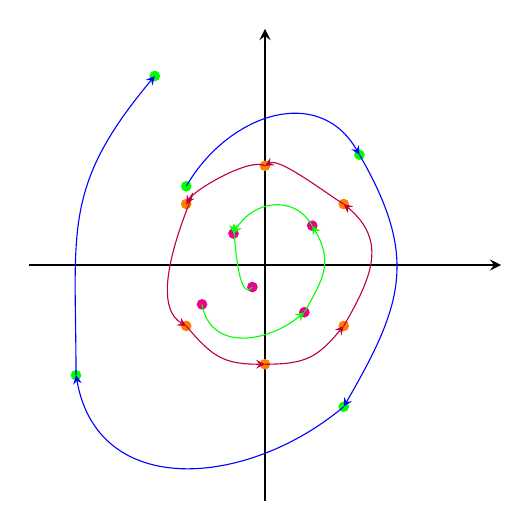
\begin{tikzpicture}[scale=2, >=stealth]
    % Axes
    \draw[->, thick] (-1.5,0) -- (1.5,0); % x-axis
    \draw[->, thick] (0,-1.5) -- (0,1.5); % y-axis
    
    % Points on horizontal axis (magenta)
    \filldraw[green] (-0.5,0.5) circle (0.03);
    \filldraw[green] (0.6,0.7) circle (0.03);
    \filldraw[green] (0.5,-0.9) circle (0.03);
    \filldraw[green] (-1.2,-0.7) circle (0.03);
    \filldraw[green] (-0.7,1.2) circle (0.03);
   
   
    % Points on vertical axis (green)
    %\filldraw[green!60!black] (0,-1) circle (0.03);
    
    \draw[blue, ->] (-0.5,0.5) to[out=60,in=120,looseness=1.2] (0.6,0.7);
    \draw[blue, ->] (0.6,0.7) to[out=300,in=60,looseness=1.2] (0.5,-0.9);
    \draw[blue, ->] (0.5,-0.9) to[out=220,in=280,looseness=1.2] (-1.2,-0.7);
    \draw[blue, ->] (-1.2,-0.7) to[out=90,in=230,looseness=1.2] (-0.7,1.2);
    
    \filldraw[magenta] (-0.2,0.2) circle (0.03);
    \filldraw[magenta] (0.3,0.25) circle (0.03);
    \filldraw[magenta] (0.25,-0.3) circle (0.03);
    \filldraw[magenta] (-0.4,-0.25) circle (0.03);
    %\filldraw[magenta] (-0.3,0.4) circle (0.03);
    \filldraw[magenta] (-0.08,-0.14) circle (0.03);

    % Arrows connecting them in a closed loop
    \draw[green, <-] (-0.2,0.2) to[out=60,in=120,looseness=1.2] (0.3,0.25);
    \draw[green, <-] (0.3,0.25) to[out=300,in=60,looseness=1.2] (0.25,-0.3);
    \draw[green, <-] (0.25,-0.3) to[out=220,in=280,looseness=1.2] (-0.4,-0.25);
    %\draw[green, <-] (-0.4,-0.25) to[out=90,in=230,looseness=1.2] (-0.3,0.4);
    \draw[green, <-] (-0.2,0.2) to[out=90,in=230,looseness=1.2] (-0.08,-0.14);
    
    \filldraw[orange] (-0.5,0.387) circle (0.03);
    \filldraw[orange] (0.5,0.387)  circle (0.03);
    \filldraw[orange] (-0.5,-0.387)  circle (0.03);
    \filldraw[orange] (0.5,-0.387)  circle (0.03);
    \filldraw[orange] (0,0.63) circle (0.03);
    \filldraw[orange] (0,-0.63) circle (0.03);

    \draw[purple, <-] (-0.5,0.387) to[out=60,in=150,looseness=0.5] (0,0.63);
    \draw[purple, <-] (0,0.63) to[out=30,in=150,looseness=0.5] (0.5,0.387);
    \draw[purple, <-] (0.5,0.387) to[out=320,in=60,looseness=1.2] (0.5,-0.387);
    \draw[purple, <-] (0.5,-0.387) to[out=230,in=0,looseness=1.2] (0,-0.63);
    \draw[purple, <-] (0,-0.63) to[out=180,in=310,looseness=1.2] (-0.5,-0.387);
    \draw[purple, <-] (-0.5,-0.387) to[out=150,in=60,looseness=1.2] (-0.5,0.387);
    
    \end{tikzpicture}
    \end{center}

\noindent
Sklep: kompleksna ravnina oz. Riemannova sfera razpade na dve disjunktni množici. \textbf{Fatoujeva}, kjer je obnašanje $f^n$ "predvidljivo" in \textbf{Juliajevo}, kjer je obnašanje $f^n$ kaotično 
\begin{align*}
\mathcal{F}_f &= \hat{\C} \slash \partial \D \\ 
\mathcal{J}_f &= \partial \D.
\end{align*}
Za formalno definicijo teh dve množic rabimo koncept normalnih družin.

\begin{definicija}
Zaporedje $(f_n)_{n\in\N} \subset \Ho(D)$ za $D \subseteq \C$, konvergira k $f \in \Ho(D)$ \textbf{enakomerno po kompaktih} na $D$, če $\forall \epsilon > 0$ in $\forall K^{komp.} \subset D$ $\exists n_0\in \N$: $\forall n \geq n_0$ in $z\in K$, velja $|f_n(z) - f(z)| < \epsilon$.
\end{definicija}

\begin{primer}
$f_n(z) = z^n$ na $\D$ konvergira enakomerno na kompaktih.
\begin{proof}[Dokaz:]
    Limita po točkah je enaka $f(z) = 0$. Izberemo poljuben kompakt $K\subset \D$.
    Zanj obstaja $r = r(K) \in [0, 1)$, da je $K \subseteq \D(0, r)$. Ker je $r < 1$, lahko naredimo oceno $\forall z\in K$:
    $$
    |f_n(z) - f(z)| = |z^n| \leq r^n \xrightarrow{n\rightarrow \infty} 0.
    $$
    tj. $\forall \epsilon > 0$ obstaja $n_0 \in \N$, da je za $n \geq n_0$: $|f_n(z) - f(z)| < \epsilon$. 
    Seveda pa enakomerna konvergenca na celem $\D$ v tem primeru ne 
    obstaja. Podobno lahko pokažemo, da gre $f_n \rightarrow \infty$ 
    enakomerno po kompaktih na $\C\backslash \overline{\D}$.
\end{proof}
\end{primer}

\begin{izrek}
Naj bo $(f_n)_{n\in\N} \subset \Ho(D)$ zaporedje ki konvergira $f_n \rightarrow f$ enakomerno po kompaktih in $D\subseteq \C$ območje. Potem je tudi $f \in \Ho(D)$ holomorfna.
\end{izrek}

\begin{proof}[Dokaz:]
Naj bo $\overline{\D(a, r)} \subset D$. Ker je $\overline{\D(a, r)}$ kompakt, 
gre $f_n \rightarrow f$ enakomerno na njem. Vsak element $f_n$ zadošča 
Cauchyjevi integracijski formuli
$$
f_n(z) = \frac{1}{2\pi i} \int_{\partial \D(a, r)} \frac{f_n(w)}{w - z} \dif w, \quad \forall z\in \D(a, r).
$$
Ker je konvergenca enakomerna, lahko zamenjamo vrstni red limite in integrala: 
$$
f(z) = \lim_{n\rightarrow \infty} f_n(z) = \lim_{n\rightarrow \infty} \frac{1}{2\pi i} \int_{\partial \D(a, r)} \frac{f_n(w)}{w - z} \dif w = \frac{1}{2\pi i} \int_{\partial \D(a, r)} \frac{f(w)}{w - z} \dif w
$$
Funkcijo na desni lahko razvijemo v vrsto okoli $z = a$, zato je holomorfna 
na $\D(a, r)$. Torej je taka tudi $f$.
\end{proof}

\begin{definicija}
Družina $\F \subset \Ho(D)$, $D \subseteq \hat{C}$ je 
\textbf{normalna na $D$}, če za vsako zaporedje $(f_n)_{n\in \N} 
\subset \F$ obstaja podzaporedje $(f_{n_k})_{k\in\N}$, ki konvergira enakomerno po 
kompaktih k neki $f\in \Ho(D)$ ali k $f\equiv \infty$.
\end{definicija}

\begin{opomba}
\hfill
\begin{itemize}
\item Normalne družine so analog kompaktnih množic v $\Ho(D) \cup \{f \equiv \infty\}$. 
Funkcijo $f \equiv \infty$ smo dodali, ker bomo obravnavali predvsem racionalne 
funkcije oz. holomorfne funkcije na $\hat{\C}$.
\item Normalnost se študira tudi v drugih razredih funkcij, v katerih pa se običajno ne dodaja $f\equiv \infty$.
\item Zadostnim oz. ekvivaletnim pogojem se reče Arzela - Ascolijevi izreki. Npr. za družino $\F \subset C([a, b])$ velja, da je normalna, če je:
\begin{enumerate}
\item[i)] enakomerno omejena tj. $\exists M > 0: |f(x)| \leq M$ $\forall x\in [a, b]$ in $\forall f\in \F$.
\item[ii)] je enakomerno enakozvezna tj. $\forall \epsilon > 0$. $\exists \delta > 0: |x - y| < \delta \Longrightarrow |f(x) - f(y)| < \epsilon$ $\forall x, y\in [a, b]$ in $\forall f\in \F$.
\item[iii)] Pri holomorfnih funkcijah $ii)$ sledi iz $i)$ zaradi Cauchyjeve integracijske formule. Zaradi kompaktnosti $\hat{\C}$ je dovolj celo lokalna omejenost. Zato se Arzela-Ascolijev izrek navadn prenese na Montelova izreka:
\begin{izrek}[Prvi Montelov izrek]
$\F \subset \Ho(D)$, $D\subseteq \hat{C}$ je normalna, če je lokalno enakomerno omejena tj. $\forall z\in D$. $\exists z\in U \subset D $ in $M > 0$, da je $|f(w)| \leq M$ $\forall w\in U$ in $\forall f\in \F$.
\end{izrek}
\end{enumerate}
\end{itemize}
\end{opomba}

\begin{definicija}
Naj bo $f \in \Ho(D)$, $D\subseteq \hat{\C}$. Njena 
\textbf{Fatoujeva množica} $\F_f$ je definirana kot množica točk
 $z\in D$, za katere obstaja okolica $U\subset D$, da je družica 
 $\{f^n \,|\, n\in \N\}$ normalna na $U$. Njena 
 \textbf{Juliajeva množica} pa je definirana kot komplement 
 $\mathcal{J}_f = D\backslash \F_f$.
\end{definicija}

\begin{primer}
$f(z) = z^2 \Longrightarrow f^n(z) = z^{2^n}$
\begin{itemize}
    \item  $|z| < 1$: konvergira enakomerno po kompaktih na 
    \item $|z| = 1$: normalnost nimamo v nobeni okolici, saj so blizu točkam, ki gredo v $\infty$ in takim, ki gredo k $0$, zato tudi, če bi obstajala limita podzaporedja, ne bi bila zvezna. 
    \item $|z| > 1$: konvergira enakomerno po kompaktih na $\hat{C}\slash\D$ $\Longrightarrow$ $\D \subset \F_f$ k $\infty$.
    \begin{proof}[Dokaz:]
    Za $K \subset \hat{C} \slash \overline{\D}$ obstaja $r > 1$, da je $\D(0, r) \cap K = \emptyset$, oz. $|z| \geq r$ za $z\in K$. \\ 
    Posledično:
    $$
    |f^n(z)| = |z^{2^n}| \geq r^{2^n} \rightarrow \infty.
    $$ 
    tj. $\forall M > 0$. $\exists n_0 \in \N$, da je $|f^n(z)| > M$ za $n \geq n_0$ in $z\in K$. Alternativno bi lahko oravnavali $\frac{1}{f^n(z)} \rightarrow 0$ enakomerno po kompaktnih. 
\end{proof}
\end{itemize}
\end{primer}


\begin{opomba}
\hfill
\begin{itemize}
\item Po konstrukciji je $\F_f$ odprta, $\mathcal{J}_f$ pa zaprta, lahko pa sta obe prazni. Primera za to sta:
\begin{itemize}
\item $f(z) = z + 1$ $\Longrightarrow$ $f^n(z) = z + n \longrightarrow \infty$ enakomerno na kompaktih na $\hat{\C}$. Torej je $\mathcal{J}_f = \emptyset$.
\item Lattesova funkcija: $f(z) = \frac{(z^2 + 1)^2}{4z(z^2 - 1)}$ ima $\mathcal{J}_f = \hat{\C}$ in $\F_f = \emptyset$.
\end{itemize}
\item Za polinome se definiciji $\mathcal{J}_f$ in $\F_f$ poenostavita, kar bomo spoznali kasneje.
\end{itemize}
\end{opomba}

\begin{izrek}
Množici $\mathcal{J}_f$ in $\F_f$ sta naprej in nazaj invariantni tj. $f(\mathcal{J}_f) = f^{-1}(\mathcal{J}_f) = \mathcal{J}_f$ in $f(\mathcal{F}_f) = f^{-1}(\mathcal{F}_f) = \mathcal{F}_f$.
\end{izrek}

\begin{proof}[Dokaz:]
Dovolj je dokazati zvezo le za $\F_f$. Naj bo $z\in U$, kjer je 
$U \subset D$, na kateri so iterati normalni. Ker je $f$ zvezna 
in odprta sta tudi množici $f^{-1}(U)$ in $f(U)$ odprti, 
seveda pa je družina $\{f^n \,|\, n\in \N\}$ normalna tudi na 
njih. Od tod sledi:
$$
f^{-1}(\F_f) \subseteq \F_f \,\,\text{ in } \,\,f(\F_f) \subseteq \F_f.
$$
Na prvo relacijo dodamo $f$ in dobimo:
$$
\F_f \subseteq f(\F_f) \Longrightarrow \F_f = f(\F_f).
$$
Posledično pa je tudi $\F_f \subseteq f^{-1}(\F_f)$, kar nam da $\F_f = f^{-1}(\F_f)$.
\end{proof}
\noindent
Povezanim komponentam $\F_f$ pravimo Fatoujeve komponente in se slikajo ena v drugo 
zaradi zveznosti in odprtosti $f$.

\begin{primer}
    Naj bo $f(z) = \frac{1}{z^2}$. Potem za iterate $f$ velja 
    \begin{align*}
    &\lim_{n\rightarrow \infty} f^{2n}(z) = \lim_{n\rightarrow \infty} z^{2^n} = 
    \Big\{\begin{array}{l}
        \infty; |z| > 1 \\
        0\,\,\,; |z| < 1
    \end{array} \\
    &\lim_{n\rightarrow \infty} f^{2n+1}(z) = \lim_{n\rightarrow \infty} z^{2^n} = 
    \Big\{\begin{array}{l}
        0\,\,\,; |z| > 1 \\
        \infty; |z| < 1
    \end{array}
\end{align*}
Vse točke $\partial \D$ so v $\mathcal{J}_f$.
\end{primer}

\section{Konjugacije in periodične točke}
Če je holomorfna funkcija $h: D \rightarrow \Omega$ obrljiva, je 
njen inverz avtomatsko holomorfen. Pravimo, da je tak $h$ biholomorfna. 
Vemo, da za $z_0 \in D$, kjer je $h'(z_0) \neq 0$ obstaja okolica $U$, 
da je $h$ zožena na $U$ biholomorfna.

\begin{primer}
Opazujemo preslikavo $h(z) = z^2$
    \begin{center}
    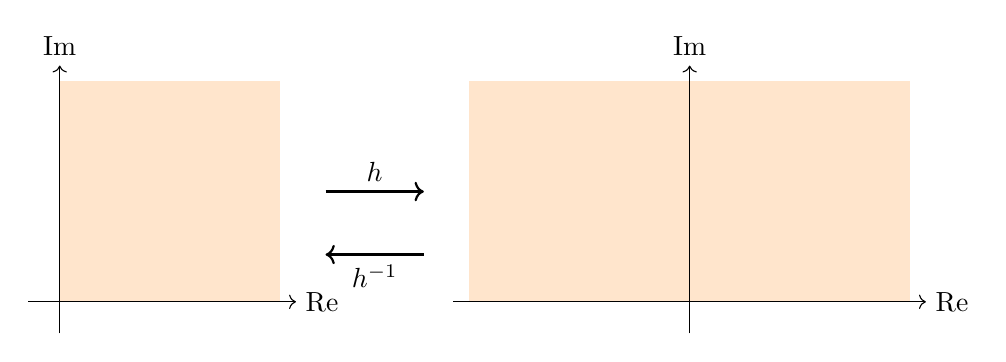
\begin{tikzpicture}[scale=2]

        % First quadrant diagram (Left)
        \begin{scope}[shift={(0,0)}]
          % Shaded first quadrant
          \fill[orange!20] (0,0) -- (1.4,0) -- (1.4,1.4) -- (0,1.4) -- cycle;
          \draw[->] (-0.2,0) -- (1.5,0) node[right] {\(\mathrm{Re}\)};
          \draw[->] (0,-0.2) -- (0,1.5) node[above] {\(\mathrm{Im}\)};

        \end{scope}
        
        % Upper half-plane diagram (Right)
        \begin{scope}[shift={(4,0)}]
          % Axes
          % Shaded upper half-plane
          \fill[orange!20] (-1.4,0) rectangle (1.4,1.4);
          \draw[->] (-1.5,0) -- (1.5,0) node[right] {\(\mathrm{Re}\)};
          \draw[->] (0,-0.2) -- (0,1.5) node[above] {\(\mathrm{Im}\)};
        \end{scope}
        
        % Arrow from first quadrant to upper half-plane
        \draw[->, thick, shorten >=5pt, shorten <=5pt] (1.6,0.7) -- node[above] {$h$} (2.4,0.7);
        
        % Arrow back
        \draw[->, thick, shorten >=5pt, shorten <=5pt] (2.4,0.3) -- node[below] {$h^{-1}$} (1.6,0.3);
        
        \end{tikzpicture}
    \end{center}
    Za $z \neq 0$ definiramo inverz 
    $$
    h^{-1}(z) = \sqrt{|z|} \cdot e^{\frac{1}{2}\arg(z)}.
    $$
    Za $z = 0$ izraz ni dobro definiran, saj okolica vsebuje 
    argumenta $0$ in $2\pi$.
\end{primer}
\begin{definicija}
Naj bo $h\in \Ho(D)$ za območje $D \subset \C$. Vrednosti $z_0$ 
pravimo \textbf{kritična točka}, če je $h'(z_0) = 0$, sliki 
$h(z_0)$ pa pravimo \textbf{kritična vrednost}.
\end{definicija}

\begin{definicija}
Naj bosta $D, \Omega \subseteq \C$ območji. Preslikavi $f:D \rightarrow D$
in $g:\Omega \rightarrow \Omega$ sta \textbf{konjugirani}, če obstaja 
biholomorfna preslikava $h: D \rightarrow \Omega$ z lastnostjo 
$h\circ f = g\circ h$. 
\end{definicija}

Ker je $f^n$ normalna na $U \subset D$ natanko tedaj, ko je 
$g^n = h\circ f^n \circ h^{-1}$ normalna na $h(U) \subset \Omega$, 
velja izrek:

\begin{izrek}
Če sta $f$ in $g$ konjugirani preko $h: D \rightarrow \Omega$, je 
$\F_g = h(\F_f)$ in $\mathcal{J}_g = h(\mathcal{J}_f)$.
\end{izrek}
To pomeni, da konjugacija ohranja karakteristični množici.

\begin{opomba}
V resnici zadošča že surjektivnost $h$ (brez omejitve na število preslik),
saj je taka preslikava lokalno biholomorfna povsod razen v disktretni 
množici. Da se pokazati, da je za nelinearno $g$ množica $\mathcal{J}_g$ 
brez izoliranih točk. Zato za kritično točko od $h$, ki leži v $z_0 \in \F_f$, 
velja tudi $h(z_0) \in \F_g$.
\end{opomba}


\begin{primer}
    Obravnavajmo preslikavo $f(z) = 3x + 2$. Fiksna točka zanjo je $z = -1$.
    Poskusimo poskrbeti, da se ta točka premakne v izhodišče.
    \begin{align*}
    &h(-1) = 0 \Longrightarrow h(z) = z + 1 \Longrightarrow h^{-1}(z) = z - 1\\
    &g(z) = h\circ f\circ h^{-1}(z) = 3z.
    \end{align*}
    Potem za Fatoujevo in Juliajevo množico dobimo 
    $$
    \F_g = \hat{\C}\backslash \{0\},\,\, \mathcal{J}_g = \{0\} \Longrightarrow 
    \F_f = \hat{\C}\backslash \{-1\},\,\, \mathcal{J}_f = \{-1\}.
    $$
    \[\begin{tikzcd}
	{-1} && {-1} \\
	\\
	0 && 0
	\arrow["f", maps to, from=1-1, to=1-3]
	\arrow["h"', maps to, from=1-1, to=3-1]
	\arrow["h"', maps to, from=1-3, to=3-3]
	\arrow["g", maps to, from=3-1, to=3-3]
\end{tikzcd}\]
\noindent
V splošnem lahko vse linearne funkcije, ki niso oblike $z \mapsto z + a$ 
transliraš v $z \mapsto a z$ za $a\in \C$.
\end{primer}
    
\begin{primer}
Poglejmo si dinamo preslikave $q_{-2} = z^2 - 2$. Vzamemo konjugacijo
$h(z) = z + \frac{1}{z}$.
\begin{itemize}
    \item $h(z) = w$ $\iff$ $z^2 - wz + 1 = 0$ ima največ $2$ rešitvi.
    \item Očitno velja $h(z) = h(\frac{1}{z})$ t.j. $\D$ in $\C \backslash$ 
    se zlepita skupaj.
    \item $|z| = 1$ $\Longrightarrow$ $z + \frac{1}{z} = z + \bar{z} = 2\Re(z)$. Preslikava 
    $h: \partial \D \rightarrow [-2, 2]$ je surjektivna, kjer je moč 
    praslike $2$, razen v točkah $z = \pm 1$.
\end{itemize}

\begin{center}
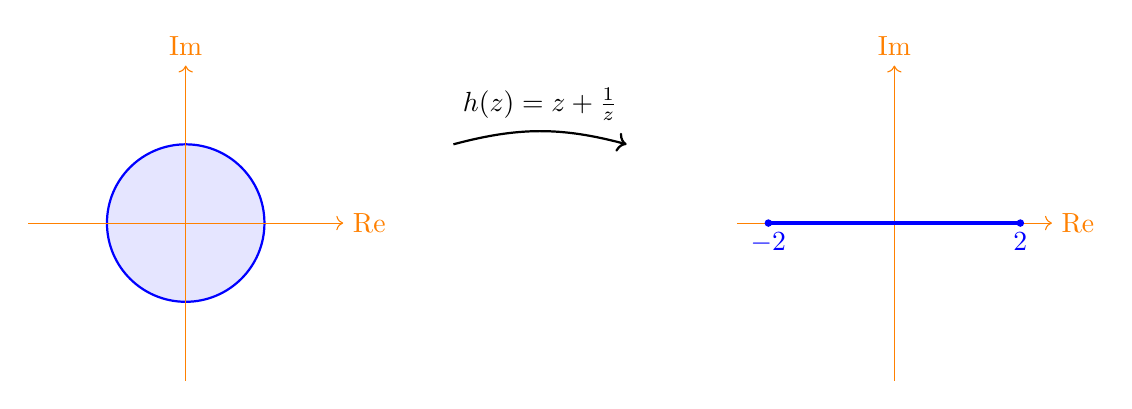
\begin{tikzpicture}[scale=2]

    % LEFT: Original complex plane
    \begin{scope}[shift={(-1.5,0)}]

        % Unit circle
        \filldraw[fill=blue!10, draw=blue, thick] (0,0) circle(0.5);
        \draw[->, orange] (-1,0) -- (1,0) node[right] {\(\mathrm{Re}\)};
        \draw[->, orange] (0,-1) -- (0,1) node[above] {\(\mathrm{Im}\)};
    \end{scope}
    
    \begin{scope}[shift={(3,0)}]
        % Axes
        \draw[->, orange] (-1,0) -- (1,0) node[right] {\(\mathrm{Re}\)};
        \draw[->, orange] (0,-1) -- (0,1) node[above] {\(\mathrm{Im}\)};
        
        % Real interval [-2, 2] (image of unit circle under h)
        \draw[very thick, blue] (-0.8,0) -- (0.8,0);
        %\node at (0,-1.3) {Image of \(|z|=1\) under \(h(z)\)};
        
        % Mark ends of interval
        \filldraw[blue] (-0.8,0) circle (0.02) node[below] {\(-2\)};
        \filldraw[blue] (0.8,0) circle (0.02) node[below] {\(2\)};
    \end{scope}
    
    % Arrow between diagrams
    \draw[->, thick] (0.2,0.5) to[bend left=15] node[above] {\( h(z) = z + \frac{1}{z} \)} (1.3,0.5);
    
    \end{tikzpicture}
\end{center}
Pokažimo, da $h$ podaja semi-konjugacijo med $f(z) = z^2$ in 
$q_{-2}$
\begin{align*}
&h \circ f(z) = z^2 + \frac{1}{z^2} \\
&g\circ h(z) = \left(z + \frac{1}{z}\right)^2 - 2 = z^2 + \frac{1}{z^2}.
\end{align*}
Sklep: $\F_{q_{-2}} = \hat{\C}\backslash [-2, 2]$ in $\mathcal{J}_{q_{-2}} = [-2, 2]$.
\end{primer}

Ker so holomorfne funkcije avtomatsko odveljive, je klasifikacija
fiksnih točk enostavna: \\
naj bo $f(z_0) = z_0$ in $f'(z_0) = \lambda$. Število $\lambda \in \C$
imenujemo \textbf{multiplikator}.
Pravimo, da je $z_0$:
\begin{itemize}
    \item Privlačan, če je $0 < \lambda < 1$
    \item Superprivlačna, če je $\lambda = 0$
    \item Odbojna, če je $|\lambda| > 1$ 
    \item Nevtralna, če je $|\lambda| = 1$.
\end{itemize}

\begin{trditev}
V okolici privlačne\slash odbojne točke je funkcija konjugirana 
preslikavi $g(z) = \lambda z$.
\end{trditev}



\section{Napolnjena Juliajeva množica}

V tem razdelku se omejimo na ne linearne polinome
$$
p(z) = a_d z^d + \dots + a_0, \quad d \geq 2.
$$

Vsi taki polinomi imajo v $z = \infty$ superprivlačno točko. Zato lahko Juliajevo 
in Fatoujevo množico definiramo na alternativen način:
\begin{itemize}
    \item  
$$
\mathcal{K}_p \coloneqq \{z\in \C \,|\, |R^n(z)| \text{ omejena} \forall n\in \N\}
$$
napolnjena Juliajeva množica.
\item 
$$
\mathcal{J}_p = \partial \mathcal{K}_p \,\text{ in }\, \mathcal{F}_p = \hat{\C}\slash \mathcal{J}_p
$$
naši karakteristični množici. 
\end{itemize}
Ker je $\infty \in \F$ in $A_p(\infty) \subset \F_p$, se ta definicija 
ujema s standardnima. To pomenim, da je dinami blizu $z = \infty$ 
konjugirana dinamiki $z \mapsto z^d$ blizu $z = 0$.\\
Slikača klopotača\\
\begin{posledica}
Za polinome stopnje $d\geq 2$ je $\mathcal{J}_p$ vedno neprazna in omejena.
\end{posledica}

\begin{proof}[Dokaz:]
    Neprazna je, ker obstaja vsaj še ena fiksna točka, ki ni $z = \infty$
    torej je $\partial A_p(\infty) \neq \emptyset$. Ostalo sledi iz dejstva, 
    da je $A_p \subset \F_p$.
\end{proof}

Ugotovili smo, da za dovolj velike $z\in \C$ orbita pobegne proti $\infty$.
Številom, ki opredeljujejo zadostno velikost pravimo \textbf{radij pobega}.

\begin{izrek}[Radij pobega]
Naj bo $P$ polinom stopnje $d\geq 2$. Naj bo 
\begin{equation}
R \coloneqq \max\Big\{\frac{3}{a_d}, \frac{2}{a_d}(|a_0| + |a_1| + \dots + |a_{d-1}|)
, 1 \Big\}.
\end{equation}
Če je $|z| \geq R$, velja 
\begin{equation}
\lim_{n\rightarrow \infty} |p^n(z)| = \infty.
\end{equation}
\end{izrek}

\begin{proof}[Dokaz:]
Naj bo $|z| \geq R$. Naredimo oceno: 
\begin{align*}
|p(z)| &= |a_d z^d + \dots + a_z + a_0| \\
&= |a_d z^d| \cdot \Bigg|1 + \frac{a_{d-1}}{a_d z} + \dots + \frac{a_1}{a_d z^{d-1}} + \frac{a_0}{a_d z^d}\Bigg| \\
&\leq \frac{|a_{d-1}|}{|a_d|\cdot |z|} + \dots + \frac{|a_0|}{|a_d|\cdot |z|^d} \\
&\leq \frac{|a_{d-1}| + \dots + |a_0|}{|a_d| \cdot |z|} \leq \frac{1}{2}.
\end{align*}

\begin{align*}
|p(z)| &= |a_d| \cdot |z|^d \cdot |1 + s| \geq |a_d|\cdot |z|^d \cdot (1 - |s|)\\
&\geq |a_d| \cdot |z|^d \frac{1}{2} \geq \frac{3}{|z|} \cdot |z|^d \frac{1}{2} \geq
&\geq \frac{3}{2} |z| \geq \frac{3}{2} R.
\end{align*}
Induktivno ugotovimo:
$$
|P^n(z)| \geq \Big(\frac{3}{2} \Big)^n \cdot R \xrightarrow{n\rightarrow \infty} \infty
$$
\end{proof}

\begin{opomba}
Ta radij ni optimalen, lahko bi še prilagajali konstanti $3$ in $2$. 
Alternativna verzija pravi npr. da je dober tudi 
$$
R = \Big\{... \Big\}
$$
\end{opomba}

Posledica tega izreka je algoritem za približno risanje $\mathcal{K}_p$, ki 
ima naslednje korake:
\begin{itemize}
    \item Določi $R$ iz izberi $N>> 1$.
    \item Naključno izbiraj točke $z_0 \in \D(0, R)$, če za vse $n\in \{1, 2, \dots, n\}$
    velja, da je $|P^n(z_0)| < R$, jih obarvaj.
\end{itemize}

Dodatno lahko razmišljamo na sledeč način. Točka $z = \infty$ je edina 
fiksna točka v komponenti $A_p(\infty)$. Torej je poleg $\partial A_p(\infty)$
edina možna limita zaporedja v $A_p(\infty).$ Izberemo $z_0 \in A_p(\infty) \slash \{\infty\}$
in tvorimo zaporedje $z_n \in P^{-n}(z_0)$ (jemljemo praslike). To zaporedje 
ne more konvergirati k $\infty$, saj gre tja zaporedje $P^n(z_0)$. Torej 
konvergira k $\mathcal{J}_P = \partial A_p(\infty)$. To pa nam da še en 
možen algoritem za približno risanje $\mathcal{J}_p$, ki mu pravimo \textbf{vzvratna iteracija}: 
\begin{itemize}
    \item Določi $R$ in izberi $N >> 1$. 
    \item Naključno izbiraj $z_0 \in \partial \D(0, R)$. Nariši množico 
    $P^{-N}(z_0)$ (kar vse praslike). 
\end{itemize}
Naš modelni primer $p(z) = z^2$ in $R = \max\Big\{ \frac{1}{|1|}, \frac{2}{|1|}\cdot 0, 1\} = 3$. 
Primerčiča:\\

\begin{izrek}[Izrek o dihotomiji]
Juliajeva množica nelinearnega polinoma je povezanan natanko tedaj, ko so vse 
kritične točke v $\mathcal{K}_p$.
\end{izrek}

\begin{opomba}
$c\in \C$ je kritična točka za $p$, če je $p'(c) = 0$. To pomeni, da je 
razvoj okoli $c$ enak:
$$
p(z) = a_0 + a_k(z-c)^k + a_{k+1}z^{k+1} + z^d a_d, \quad k \geq 1.
$$
To pomeni, da lokalno oz. za vrednosti blizu $z = c$ funkcija $p$ 
"deluje kot" $z \mapsto z^k$ v posebnem, na okolici take točke $p$ ni
injektivna.
\end{opomba}

\begin{primer}
Oglejmo si primer $z \mapsto z^2$ in tri tipe krožnic ter njihovih praslik: 
kul slikice\\
Morala: če krožnica trči v kritično vrednost, je njena praslika topološko 
ekvivalentna osmici, krožnice v njej pa imajo dve nepovezani komponenti v 
prasliki.
\end{primer}

\begin{proof}[Dokaz(ideja):]
Ločimo dva primera:
\begin{enumerate}
    \item v $A_p(\infty)$ ni kritičnih točk in posledično tudi kritičnih vrednosti ne. 
    Za poljuben $r \geq R$, kjer je $R$ radij pobega, je množica $P^{-n}(\partial \D(0, r))$, 
    $n\in \N$, sklenjena krivulja brez samopresečišč (krožnica v topološkem smislu).
    V limiti pa dobimo $\mathcal{J}_p$, ki je povezana. 
    \item Če $A_p(\infty)$ vsebuje kritično točko in posledično tudi kritično vrednost 
    , potem bo praslika križnice $D(0, |p(c)|)$ unija več topoloških krožnic s 
    skupnim presečiščem. Manjše krožnice pa bodo razpadle na več komponent. \\
    Neki lepega
\end{enumerate}
\end{proof}

\section{Drugi Montelov izrek}

V tem razdelku bomo spoznali enega bolj pomembnih izrekov v kompleksni analizi, 
ki močno opredeli lastnosti množice $\mathcal{J}_R$. Omejili se bomo 
na racionalne funkcije stopnje $d \geq 2$. 

\begin{izrek}[Drugi Montelov izrek]
Če obstajo vrednosti $a, b, c \in \hat{\C}$, ki so različne. ter za družino 
$\F \{R: D \subseteq \hat{\C} \rightarrow \hat{\C}$ \,|\, R \text{ racionalna}\} 
velja $\{a, b, c\} \cap R(D) = \emptyset$ za vsak $R \in \F$, potem je 
$\F$ normalna. 
\end{izrek}

\begin{opomba}
\begin{itemize}
    \item Izrek velja tudi za družine meromorfnih funckij na $D \subset \C$ tj. 
    za funkcije brez bistvenih singularnosti.
    \item Izrek je pogosto podan za družine holomorfnih funkcij $\F \subset \O(D)$, 
    za $D \subset \C$, takrat je dovolj, da izpusti dve točki $a, b \in \C$, saj 
    za $c$ vzamemo $\infty$ (elementi $\F$ nimajo polov).
\end{itemize}
\end{opomba}

\begin{proof}[Dokaz(ideja).]
Kjučen del dokaza je obstoj surjektivne holomorfne preslikave 
$$
h: \D \rightarrow \hat{\C}\backslash \{0, 1, \infty\},
$$
ki nima kritičnih točk oz. je krovna projekcija tj. zožitev $h$ na vsako 
komponentno take praslike je biholomorfna. Od tu dalje brez škode za splošnost 
predpostavimo, da so $a = 0$, $b=1$ in $c = \infty$. Če to ni res, vse 
$R \in \F$ konjugiramo z ustrezno Möbiousovo preslikavo. 

Sedaj je preslikave "dvignemo na krov"
\end{proof}

Obravnavajmo dinamiko $f:D\subseteq \hat{\C} \rightarrow \hat{\C}$. 
Drugi Montelov izrek nam porodi številne posledice,  še posebaj 
za Juliajevo množico, kjer nimamo normalnosti.

\begin{posledica}[Množica izjemnih točk]
Naj bo $R$ racionalna funkcija, stopnje $d\geq 2$, ter $x\in \mathcal{J}_R$
in $U_z \in \hat{\C}$ njena okolica. Množica 
$$
E_R(U_z) \coloneqq \hat{\C} \backslash \bigcup_{n=0}^\infty R^n(U_z)
$$
vsebuje največ $2$ točki.
\end{posledica}

To je direktna posledica izreka.\\
slika frika\\
$E_R$ lahko izpusti največ $2$ točki, scer bi bila normalna.

\begin{primer}
    \hfill
\begin{itemize}
    \item $p(z) = z^2$. V tem primeru je $E_R(U_z) = \{0, \infty\}$ za vse 
    $U_z$ in $z\in \mathcal{J}_p$.\\
    slikica
    \item $p(z) = z^2 - 2$. Sedaj dobimo $E_p(U_z) = \{\infty \}$ za vse 
    $U_z$ in $z\in \mathcal{J}_p$.\\
    slikica mikica
\end{itemize}
Z nekaj dodatne analize se izkaže, da sta to do konjunkcije natančno 
primera z neprazno množico izjemnih točk. Natančneje, za $z\in \mathcal{J}_R$ 
definiramo 
$$
E_R(z) \coloneqq \bigcup_{U_z \text{ okolica}} E_R(U_z). 
$$
Da se pokazati:
\begin{itemize}
    \item če je $|E_R(z)| = 2$, je $R$ konjugirana $z \mapsto z^d$, $d \geq 2$.
    \item Če je $|E_R(z)| = 1$, je $R$ konjugirana polinomu stopnje $d \geq 2$, 
    za katere je $E_R(z) = \{\infty\}$ za vse $z\in \mathcal{J}_p$. 
\end{itemize}
V obeh primerih je $E_R(z)$ neodvisna od točke $z\in \mathcal{J}_p$,
zato je to tudi res v splošnem in lahko definiramo $E_R \coloneqq E_R(z)$
za poljuben $z\in \mathcal{J}_R$. Tej množici pravimo \textbf{množica izjemnih 
točk} in vedno velja $E_R \subset \F_R$.
\end{primer}

\begin{posledica}[Juliajeva množica z neprazno notranjostjo]
Naj bo $R$ racionalna stopnje $d \geq 2$. Če ima $\mathcal{J}_R$
 neprazno notranjost, je $\mathcal{J}_R = \hat{\C}$.
\end{posledica}

\begin{proof}[Dokaz:]
Če ima $\mathcal{J}_R$ neprazno notranjost, obstaja odprta množica 
$U \subset \hat{\C}$, ki ni prazna in je $U \subset\mathcal{J}_R$. 
Po prejšnji posledici ima:
$$
\hat{\C} \backslash \bigcup_{n=1}^\infty R^n(U)
$$
največ $2$ točki. Ker je $\mathcal{J}_R$ naprej in nazaj invarintna, 
velja $R^n(U) \subset \mathcal{J}_R$ za vsak $n\in \N$. To pomeni, da je:
$$
\hat{\C} \backslash E_R = \bigcup_{n=1}^\infty R^n(U) \subseteq \mathcal{J}_R. 
$$
Torej za zaprtje velja:
$$
\overline{\hat{\C} \backslash E_R} = \hat{\C} \subseteq \overline{\mathcal{J}}_R = \mathcal{J}_R.
$$
\end{proof}

\begin{opomba}
V uvodu smo povedali, da teka funkcije dejansko obstajajo (Lattesova preslikava).
\end{opomba}


\begin{posledica}[Goste praslike]
Naj bo $R$ racionalna stopnje $d \geq 2$. Za vsako $z\in \mathcal{J}_R$
je množica 
$$\bigcup_{n=1}^\infty R^{-n}(\{z\})$$
gosta v $\mathcal{J}_R$.
\end{posledica}

\begin{proof}[Dokaz:]
Za vsako $z \in \mathcal{J}_R$ vemo, da $z\not\in E_R \subset \mathcal{F}_R$.
Če izberemo okolico $U_z \subset \hat{\C}$ trdimo, da za poljubno 
drugo točko $z' \not\in E_R$ obstaja $n\in \N$, da je $z' \in \R^n(U_z)$.\\
neki malega\\
Če je dodatno $z' \in \mathcal{J}_R$, ima tudi $R^n(U_z)$ neprazen presek z 
$\mathcal{J_R}$.\\
še nekaj malo večjega\\
Torej je: $\mathcal{J}_R \subseteq \overline{\bigcup_{n=1}^\infty} R^{-n}(z')$.
Če pa izberemo $z' \in \mathcal{J}_R$, pa zaradi invariantnosti velja 
tudi obratna inkluzija
$$
\bigcup_{n=1}^\infty R^{-n}(z') \subseteq \mathcal{J}_R.
$$
Torej to drži tudi za zaprtje.
\end{proof}

\begin{posledica}[Kaotičnost na $\mathcal{J}_R$]
Naj bo $R$ racionalna stopnje $d \geq 2$. Potem je zožitev 
$R: \mathcal{J}_R \rightarrow \mathcal{J}_R$ kaotična v smislu 
Devaneya.
\end{posledica}

\begin{proof}[Dokaz:]
\begin{enumerate}
    \item[c1)] Gostost periodičnih točk: sledi iz $\overline{Rep}(R) = \mathcal{J}_R$
    t.j. že zgolj odbojne točke so goste.
    \item[c2)] Tranzitivnost: naj bosta $u, V \subset \mathcal{J}_R$ odprti 
    glede na relativno topologijo t.j. $\exists U', V' \subseteq \hat{\C}$
    odprti, da je $U = \mathcal{J}_R \cap U'$ in $V = \mathcal{J}_R \cap V'$. 
    Iščemo $z\in U$ in $n\in \N$, da bo $R^n(z) \in V$. Najdemo ga po prejšnji 
    posledici. Vzamemo katerikoli $w\in V$. Zaradi gostosti praslik, obstaja 
    $R^{-n}(\{w\}) \cap U \neq \emptyset$. Torej obstaja tudi $z\in U$, da je 
    $R^n(z) = w \in V$.
    \item[c2)] sledi iz $c1)$ in $c2)$, ker je $R$ zvezna.
\end{enumerate}
\end{proof}

\begin{posledica}
Naj bo $R$ racionalna stopnje $d \geq 2$. Potem za vsako $z\in \mathcal{J}_R$
in vsako okolico $U_z$ obstaja $z'\in \mathcal{J}_R \backslash \{z\} \cap U_z$.
\end{posledica}

\begin{proof}[Dokaz:]
Naj bo $z\in \mathcal{J}_R$ in $U_z$ poljubna okolica. Ločimo dva primera 
\begin{enumerate}
    \item[i)] $z$ ni periodična: izberemo poljuben $w \in R^{-1}(\{z\})$\\
    spet slika\\
    Zaradi neperiodičnosti imamo: 
    $$
    R(w) = z \,\, \text{ in } \,\, R^n(z) \neq w \,\,\, \forall n\in \N.
    $$
    Vendar pa po posledici $3$ obstaja tudi $z' \in U_z$ in $m\in \N$, 
    da je $R^m(z') = w$. Po konstrukciji $z' \neq z$.
    \item[ii)] zapiski.
\end{enumerate}
\end{proof}

\section{Fatou-Sullivanov izrek}

Ugotovili smo, da je $\F_R$ odprta ter naprej in nazaj invariantna.
To pomeni, da se njene komponentne za povezanost slikajo ena 
v drugo. V principu se nam lahko zgodijo $4$ stvari:\\
4 horsemen of the apocalypse\\


\begin{izrek}
Racionalna funkcija stopnje $d \geq 2$ ima $0, 1, 2$ ali $\infty$
Fatoujevih komponent.
\end{izrek}

\begin{proof}[Dokaz:]
    Predpostavimo, da je komponent končno. Trdimo, da so takrat 
    vse periodične ali fiksne t.j. ne more se zgoditi predperiodičen primer.\\
    sdaCC\\
    t.j. obstaja $\tilde{U} \subset \F_R$ komponenta in $k < n\in \N$, da je 
    $$
    U = R^n(\tilde{U}) = R^k(\tilde{U}).
    $$
    $$
    R^{n-k}(U) = R^{n-k}(R^k(\tilde{U}) = R^n(\tilde{U})) = U     
    $$
    $\Longrightarrow n-k$ je kandidat za periodo (morda je manjša).
    Sklep je, da obstaja $N\in \N$, da je 
    $$
    R^N(U) = U \,\,\text{ za vse komponente $\F_R$}.
    $$
    To je res, ker jih je po predpostavki končno in lahko izberemo 
    najmanjši skupni večkratnik period.

\end{proof}


\end{document}